\documentclass[12pt, a4paper]{article}
\usepackage{amsmath,amsfonts,amssymb,amsthm,mathtools}
\usepackage{fontspec}        
\setmainfont{Roboto} 
\usepackage{unicode-math}    
\setmathfont{Asana Math}  
\usepackage{polyglossia}      
\setdefaultlanguage{russian}  
\setotherlanguage{english}
\usepackage{graphicx}

\author{Маликова Ольга}
\title{Домашнее задание 1}
\date{\today}

\begin{document}

\maketitle

\section{10 фактов о себе}

\begin{enumerate}
\item Увлекаюсь фотографией почти 2 года. Больше всего люблю фотографировать портреты людей и мечтаю освоить плёночный фотоаппарат. 
\item Боюсь щекотки и лягушек :)
\item Научилась кататься на велосипеде только в 12 лет.
\item Люблю весну.
\item Больше люблю дарить подарки, чем получать.
\item При виде крови падаю в обморок. И такая особенность в себе почему-то нравится :)
\item Руководствуюсь больше эмоциями, чем разумом. Порой излишне впечатлительная.
\item Если что-то становится мейнстримом, сразу теряю к этому интерес.
\item Любимая антиутопия "Мы" Евгения Замятина.
\item Люблю своё полное имя.
\end{enumerate}

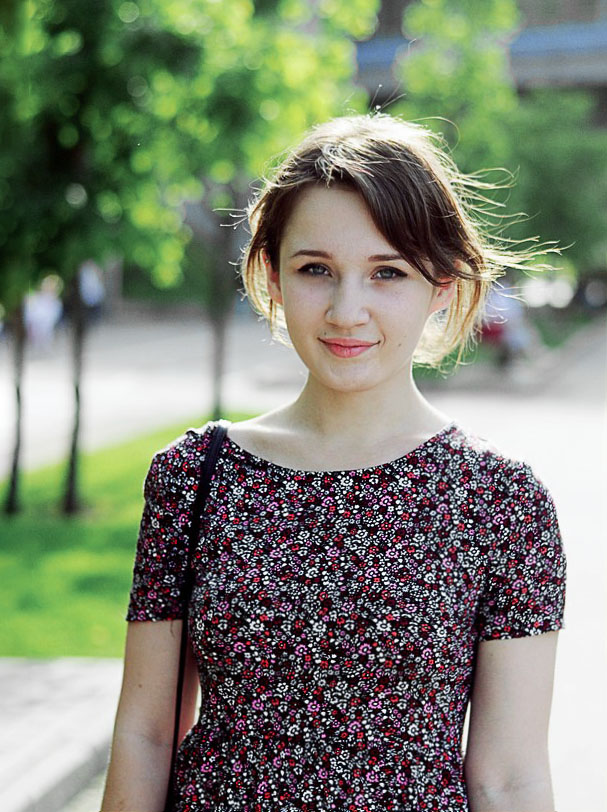
\includegraphics[width=15 cm]{olia.jpg}

\section{Формулы}

\subsection{Любимые формулы}

\begin{enumerate}
\item Определитель квадратной матрицы третьего порядка 
\begin{equation}
\begin{aligned} 
 \begin{vmatrix}
  a_{1,1} & a_{1,2} & a_{1,3} \\
  a_{2,1} & a_{2,2} & a_{2,3} \\
  a_{3,1} & a_{3,2} & a_{3,3}  \\
 \end{vmatrix} = a_{1,1} \cdot a_{1,2} \cdot a_{1,3} + a_{1,2} \cdot a_{2,3} \cdot a_{3,1} + \\
+ a_{1,3} \cdot a_{2,1} \cdot a_{3,2} - a_{3,1} \cdot a_{2,2} \cdot a_{1,3} - \\
  - a_{2,1} \cdot a_{1,2} \cdot a_{3,3} - a_{1,1} \cdot a_{3,2} \cdot a_{2,3}
 \end{aligned} \tag{æ}
\end{equation}

\item Бином Ньютона
\begin{equation}
\begin{aligned} 
(a + b)^n = C_n^0 \cdot a^n \cdot b^0 + C_n^1 \cdot a^{n-1} \cdot b^1 + C_n^2 \cdot a^{n-2} \cdot b^2 + ... \\
 ... + C_n^{n-1} \cdot a^1 \cdot b^{n-1}+ C_n^n \cdot a^0 \cdot b^n = \sum_{k=0}^n C_n^k \cdot a^{n-k} \cdot b^k 
\end{aligned} \tag{ææ}
\end{equation}

\item Формула бесконечно убывающей геометрической прогрессии
\begin{equation}
S = \frac{b_1}{1 + q} \tag{æææ}
\end{equation}

\item Второй замечательный предел
\begin{equation}
\lim_{n \to \infty} \frac{\sin x}{x} = 1 \tag{ææææ}
\end{equation}

\item Интеграл Эйлера-Пуассона 
\begin{equation}
\int_0^{\infty} e^{-x^2} dx = \frac{\pi}{2} \tag{æææææ}
\end{equation}

\subsection{Нелюбимая формула}

\item Дисперсия оценки коэффициента $\hat \beta_1$, полученной МНК
\begin{equation}
\sigma_{\hat \beta_1} = \frac {Var((x_i - \mu_x)\cdot u_i)}{n \cdot (Var (x_i))^2} \tag{ææææææ}
\end{equation}
\end{enumerate}

 Формулу \ref{æ} я полюбила после того, как узнала лёгкий способ её запоминания. 
 Формулы \ref{ææ} и \ref{æææææ} напоминают мне о теории вероятностей и математической статистике, которые вёл Василий Павлович, а это всегда приятные воспоминания.
  Формулу \ref{æææ} люблю за её простоту и широту применения. 
Ну и как же без одного из двух замечательных пределов? Мне больше нравится второй замечательный предел \ref{ææææ}, наверное из-за наличия функции синус. 

С нелюбимой формулой всё просто. Я не люблю \ref{ææææææ}, потому что не могу запомнить и понять суть её выведения. 
\end{document}